\chapter{Word2vec for Document Classification of German language business document}
\label{chap:rel_word2vec_doc_classification}

% Introduction 
%  - Promises of deep learning
%  - Help many task
%  - Document classification is an interesting problem because there is a
%  standard methdology to use word vector representation
%  Structure of the chapter
%  Gini document infraestructure (qucik description of Count Dooku)
%  Gini dataset and document classification dataset.
%  Description of the current implementation
%  BoW word model
%  Word2Vec document mean vector representation
%  Comparisson of the model
%  Different Feature visualization
%  Conclusion and Future work. 
%   - Using individual features will make always hard to work with variable
%   - Sized documents - that is definitive.

\section{Introduction}
\label{sec:w2v4tc_intro}

One of the motivation of feature learning is to be able to
obtain useful representation that will improve existing task. In the case of
\ac{NLP} word vector features have been shown to improve existing taks such
as \ac{NER}, Chunking and Sentiment Analysis \cite{Turian:2010:WRS:1858681.1858721}
\cite{DBLP:journals/corr/abs-1103-0398}  and have shown promising results in
fields as machine translation and speech processing \cite{collobert:2008}
\cite{DBLP:journals/corr/MikolovLS13}.  

In the field of \ac{TC} there have
not been much work of improving this task by using word vector representations. There are many reason
fo this. One can be that many of the current methods work well enough, in particular those
based on the \ac{VSM} \cite{Sebastiani02}. Another reason might be that that
when using word representation each word get a $n$-dimensional vector
representation representation, therefore a large document could be only
represented as big matrix,  and current methods work only with vector
representation od document. However there has been previous work using word
vector for short text classification, namely sentiment analysis
\cite{maas2011learning} . Sentiment Analysis can be seen as a variation of
\ac{TC}. In fact in the aforementioned work the use the traditional
approaches for \ac{TC} to train the sentiment predictor.  In this work the
performance  word vector representations based on the \textit{Word2vec} model 
are compared against other features  in the context of classifying  business-related German language
documents. The objective is therefore to improve the existing classifier by
using the learned word vector features. However, as a byproduct other more
traditional features are evaluated to validated whether they work better. 

So, the objective of this part of the work is two-fold:  One  hand the
evaluation of the word vector representation and on the other find a better
features for the existing classifier, even if they are not based on the
learned word representation.

The rest of the chapter is divided as follows: The first part describes 
the company's  document platform, the requirements and challenges behind this
particular document classification task. The second the part describes the different features
used and the classification algorithms used while explaining the limitation
faced.  The third and final  part discusses the most important results as
well as well as the future work. 

\begin{figure}[h]
    \centering
    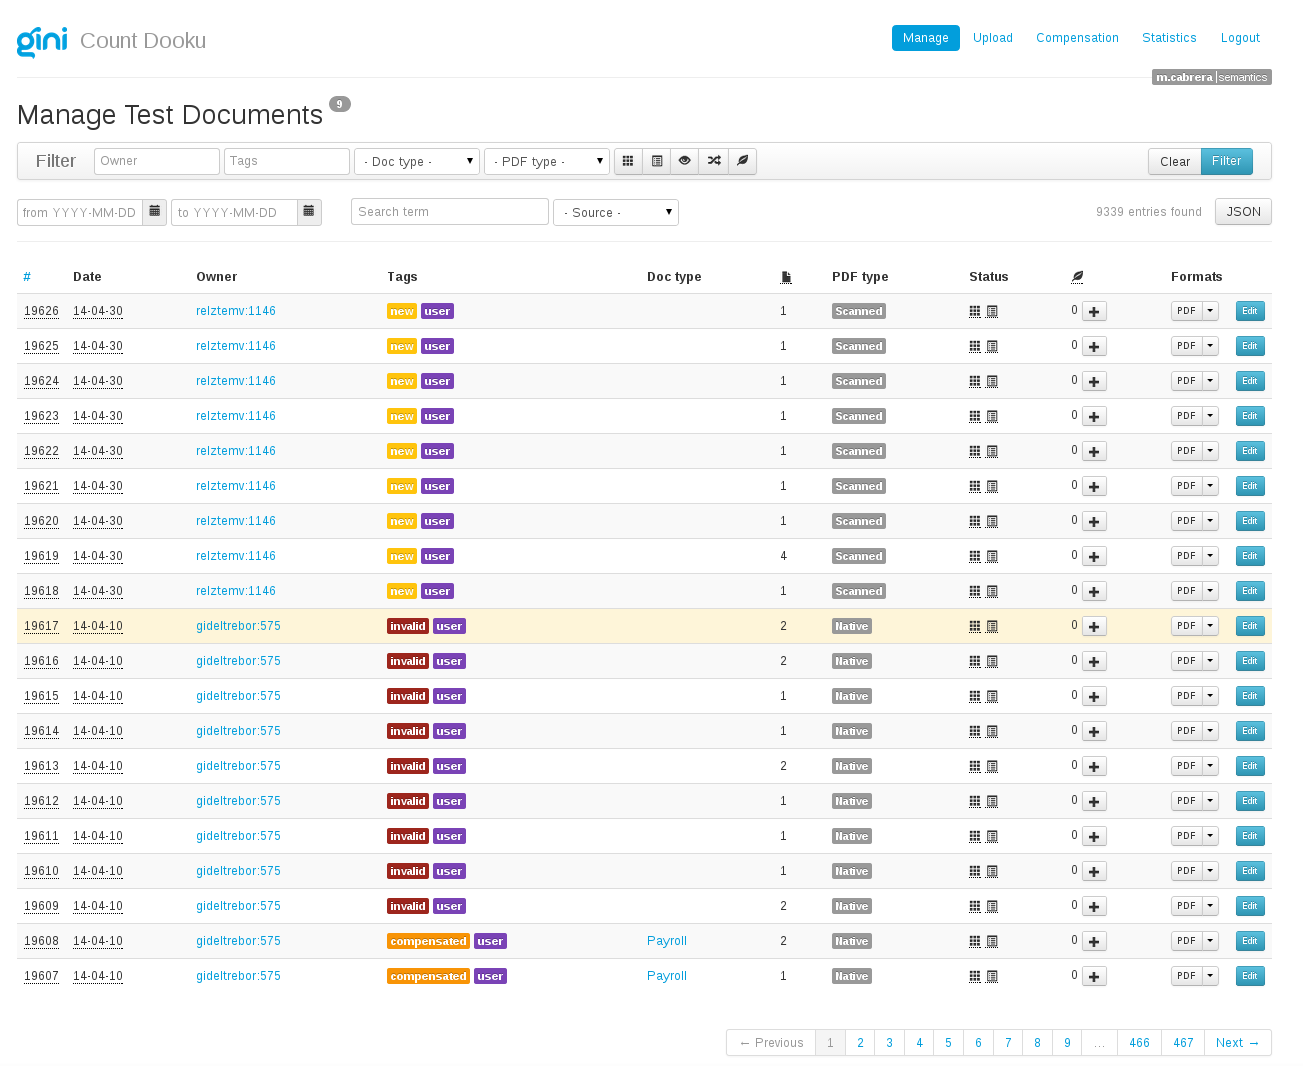
\includegraphics[width=\textwidth]{images/001-dooku-screenshot.png}
    \caption{Dooku - Gini document storage platform.}
    \label{fig:dooku_screenshot}
\end{figure}

\section{Gini document platform}
\label{sec:gini_doc_platform}

Gini currently owns a database  German language document. These documents 
are personal and business related documents that have been bought 
from  persons all over Germany. Document types are very broad and go from
long insurance contracts to short remittance slips. These document are stored
in a central system database that can be accessed via an  \texttt{API}.
Document can be either \textit{native} or \textit{scanned}. The document
\textit{native} that are native are orignal digital document. (e.g. PDF document) that
are uploaded to the system. \textit{Scanned} documents on the other hand, are
uploaded from an image obtained a scanner or a camera (e.g. a mobile phone
camera). Given the variability of the capture devices for the scanned
documents, the quality of such images is not regular among all the documents.
This is important to consider, given that after being uploaded all the
documents are processed using a \ac{OCR} solution, so the quality of the
images affect the the accuracy with which the text is extracted from. 
After the text has been extracted, it is stored  along with
the position of the words on the page; font size and style,  and other information a into a database using a custom
\textsc{XML} format.  Besides this information, a document is also assigned
\textit{tags} or labels, that when querying for particular characteristic
(e.g. quality, source, etc.) help filter the results. Figure
\ref{fig:dooku_screenshot} shows a screen-shot of the application with the
most important columns.


After being stored and preprocessed, this document are annotated by a human.
The annotations include labels such as  \textit{sender name}, \textit{bank
  account} (in the case of financial documents), \textit{amount to pay} and
\textit{document type} (\ac{DocType}). Using this annotation several
machine leaning algorithm are trained.  These classifier are then exposed to
clients also via an \texttt{API}. Table \ref{tab:list_gini_doctypes} shows the
complete list of \ac{DocTypes} available in the system and their description.


\section{The Gini Document Classifier}  
\label{sec:gini_doctype_classifier}

One of the functionality that Gini offer to their customer is document
classification.  As mentioned in the previous section this is done using
machine learning on top of the annotations made by humans. In the particular
case of the \ac{DocType} classifier, it is implemented using \ac{SVM} using
handcrafted features such as the appearance of a particular word, the font
of specific words, the number of pages of the documents, etc. This features
once constructed are fed into the \ac{SVM} implementation to train classifier. the
classifier is then exposed through a Web service.

The particular implementation of the \ac{SVM} is based on \texttt{Java}
implementation of the popular \texttt{LIBSVM} \cite{CC01a} using a
\texttt{RBF} Kernel.  The training is done using grid search and the best
model in 10-fold cross-validation with all the training data available is
taken.

There are some external an internal challenges that this classifier is faced
with:

\begin{itemize}
\item The quality of the data: As much of the data comes from varying degree
  of capture devices, the quality of the OCR is not perfect, thus producing a
  lot of noise in the stored text.
\item Feature generation and extension: Every time a new document type is
  required to be supported, a manual analysis of the document type should be
  done with the purpose of identifying what features are important and then
  these are added to the document.
\item No validation of the classifier is done on a validation set and quality
  is measured on documents belonging to the training set. This fundamental
  flaw, albeit obvious in a scientific setting, is many times overlooked in
  the industry.
\end{itemize}

Taking in consideration all these challenges, the objective is then to design
a better classifier that allow, at least partially, solve the
aforementioned issued.



\section{Experimental Setup}
\label{sec:w2vec_doctype_experimental_setup}

As mentioned in the introduction, three different approaches are going to be
compared, namely:

\begin{itemize}
\item The current \ac{SVM} implementation with the handcrafted features.
\item A new \ac{SVM} implementation using \ac{BOW} features.
\item A new \ac{SVM} implementation using \textit{Word2vec} word vector as features.
\end{itemize}

The classification algorithm is kept while the
evaluation real evaluation is on the features. The idea  is to verify
that in fact better features account for better classification. The following
sections describe each of the features and the specific od the algorithm. 


\subsection{Gini Document Database and Dataset Description}
\label{sec:gini_db_dataset_desc}
  
Section \ref{sec:gini_doc_platform} described briefly the platform where
document Gini owned resided. This section described the specific of the
documents used for training the classifier. 

Gini database of documents consists of approximately 9339 different types of
document, from these only 2685 are used to train the document classifier.
Table \ref{tab:doctype_classifier_classes} show the distribution of the data
set among the classes. As can be seen from the data set, not all classes
used. Furthermore, there is a class called \textit{Other} that include
documents that do not fall into any of the categories listed. It is also a
unbalanced data set, having with number of intances per class ranging from 69
to 650. All the document are not used in the data set because as of right now
it is not necessary to classify all of other classes (creating thus a large
unbalanced \textit{Other} class). Additionally, other document are not
annotated or annotated wrongly, that is, they are correct document but has
not been properly annotated with the correspondent \ac{DocType}.


\begin{table}[h]

  \centering
  \caption{Distribution of document type in  Gini \ac{DocType} classifier training set.}
  \label{tab:doctype_classifier_classes}

\small
\begin{tabular}{|l|c|}
\hline
 \textbf{Document Type}    &  \textbf{\# Instances}  \\
\hline
 CreditCardStatement  &           158  \\
 Other                &           650  \\
 BankStatement        &           369  \\
 Contract             &           178  \\
 InsurancePolicy      &           105  \\
 Payroll              &            69  \\
 Invoice              &           570  \\
 Reminder             &           596  \\
\hline
 Total                &          2685  \\
\hline
\end{tabular}
\end{table}

As mentioned mentioned previously, there was not an official test set used to
evaluate the classifier performance. Therefore a new one was defined using a
stratified random selection of 20\% original  set for the testing and the
other 80\% for training, ending up with 2156 documents for training  539 for
testing. The same documents are used to evaluate all the classifier /
features.


\subsection{Handcrafted Features}
\label{sec:sub_w2v4tc_current_features}

As mentioned back in section  \ref{sec:gini_doctype_classifier} the current
Gini document classifier is based  \texttt{LIBSVM} \cite{CC01a} using 
\texttt{RBF} Kernel.   The features used to rain this classifier are
handcrafted features that count then number of words (actually the matches of
specific regular expressions) in the text, the font size of some
words, the digit character ration, the average font size, etc. In total 701 features like these are used.
 

\subsection{\ac{BOW} Features}
\label{sec:sub_w2v4tc_bow_features}

For the \ac{BOW} features, the traditional \ac{tf-idf}  
\cite{Salton88term-weightingapproaches}\cite{Sebastiani02} discussed in
section [LINK TO RELATED WORK] is used as features. For the actual feature
extraction the \texttt{TfidfTransformer} from \texttt{Scikit-learn}
\cite{scikit-learn}  was used ending up with 55122-dimensional sparse
vectors.
  
% The training is done using grid search and the best
% model in 10-fold cross-validation with all the training data available is
% taken.






% - Stored Dookud
% - Stored as DocXML not only text but also location information of words.
% - Two ways to get the text from the document {Native, Scanned (e.g.)}

%  approach as well as the most
% important results. It includes  a performance comparison of the word vectors in German with their counterpart in English as well as  the evaluation of  some corpus
% preprocessing approaches that might affect the performance of the word
% representation for German.


      %\caption{List of document types available in Gini Dataset}
      %\label{tab:list_gini_doctypes}
%\begin{tabular}{|c|p{8cm}|}


% \begin{longtable}[h]{|l|p{9cm}|}
% \caption[List of document types available in the Gini Dataset]{List of document types available in the Gini Dataset} \label{tab:list_gini_doctypes} \\
% \hline DocType code & Description \\
% \hline Administrative\_offence                  &  Administrative offence - Administrative Rechnungen, wie z.B. Strafzettel, Bu{\ss}geldbescheide      \\
%  admission\_ticket                        &  Admission ticket -  Eintrittskarte                                                                \\
%  airline\_ticket                          &  Airline ticket -  Flugticket (Boardkarte, Buchung)                                                \\
%  bank\_statement                          &  Bank statement -  Kontoauszug                                                                     \\
%  confirmation\_of\_termination            &  Confirmation of termination -  K\"{u}ndigungsbest\"{a}tigung                                  \\
%  contract                                 &  Contract -  Vertrag                                                                               \\
%  contract\_confirmation                   &  Contract  confirmation -  Best\"{a}tigung Vertrag (alle Dom\"{a}nen)                          \\
%  contract\_energy                         &  Contract  energy  - Energie (Vertrag)                                                             \\
%  contract\_extension                      &  Contract  extension -  Vertragsverl\"{a}ngerung                                                 \\
%  contract\_insurance\_automobile          &  Contract insurance automobile -  Kfz-Versicherung (Vertrag)                                       \\
%  contract\_insurance\_household           &  Contract insurance household -  Hausratversicherung (Vertrag)                                     \\
%  contract\_insurance\_legal\_costs        &  Contract insurance legal costs - Rechtsschutz (Vertrag)                                           \\
%  contract\_insurance\_third\_party\_risk  &  Contract insurance third party risk  - Haftpflicht (Vertrag)                                      \\
%  contract\_telco                          &  Contract telco -  Telko (Vertrag)                                                                 \\
%  credit\_card\_statement                  &  Credit card statement - Kreditkartenabrechnung                                                    \\
%  credit\_note                             &  Credit note -  Gutschrift                                                                         \\
%  delivery\_note                           &  Delivery note -  Lieferschein                                                                     \\
%  insurance\_policy                        &  Insurance policy -  Versicherungsunterlagen                                                       \\
%  invoice                                  &  Invoice - Rechnung                                                                                \\
%  lease\_contract                          &  Lease contract -  Mietvertrag Leasingvertrag                                                      \\
%  letter                                   &  Letter  Brief - (interessante Doks f\"{u}r die es keinen DocType gibt)                          \\
%  medical\_finding                         &  Medical finding - Medizinischer Befund                                                            \\
%  medical\_insurance                       &  Medical insurance -  Krankenversicherungsdokument                                                 \\
%  notice\_of\_termination                  &  Notice of termination -  K\"{u}ndigung                                                          \\
%  offer                                    &  Offer -  Angebot                                                                                  \\
%  order\_confirmation                      &  Order confirmation  - Bestellbest\"{a}tigung, Auftragsbest\"{a}tigung                         \\
%  payroll                                  &  Payroll -  Gehaltsabrechnung                                                                      \\
%  receipt                                  &  Receipt  - Kassenzettel                                                                           \\
%  reminder                                 &  Reminder  Mahnung                                                                                 \\
%  remittance\_slip                         &  Remittance slip -  \"{U}berweisungstr\"{a}ger                                                 \\
%  return\_form                             &  Return form -  R\"{u}ckgabeformblatt (z.B. ecommerce amazon)                                    \\
%  social\_security\_statement              &  Social security statement -  Sozialversicherung, Meldebescheinigung zur Sozialversicherung        \\
%  statement\_energy\_consumption           &  Statement energy consumption -  Verbrauchsabrechnung (Strom, Gas, Wasser, etc)                    \\
%  statement\_pension                       &  Statement pension -  Rentenbescheid, Rentenversicherungsunterlagen                                \\
%  stock\_document                          &  Stock document -  Wertpapierdepotausz\"{u}ge, Dividendenabrechnungen, Orderbest\"{a}tigungen  \\
%  tax\_assessment                          &  Tax assessment  Steuerbescheid                                                                    \\
%  tax\_document                            &  Tax document -  Lohnsteuerbescheinigung, Best\"{a}tigung f\"{u}r die Steuererkl\"{a}rung    \\
%  tax\_return                              &  Tax return -  Steuererkl\"{a}rung                                                               \\
%  taxi\_receipt                            &  Taxi receipt - Taxi-Quittung                                                                      \\
%  terms\_and\_conditions                   &  Terms and conditions -  Gesch\"{a}ftsbedingungen                                                \\
%  travel\_expense\_report                  &  Travel expense report - Reisekostenabrechnung     \\             \hline                          
% \end{longtable}



%%% Local Variables: 
%%% mode: latex
%%% TeX-master: "../main.tex"
%%% End: